\pdfoutput=1
\RequirePackage{amsmath}
\documentclass[iop, apj]{emulateapj}
\usepackage[varg]{newtxmath}
\usepackage{newtxtext}
\usepackage[spanish,es-minimal,english]{babel}
\usepackage[utf8]{inputenc}
\usepackage{natbib}
\usepackage{microtype}
\usepackage{hyperref}
\graphicspath{ {figs/}, {../}, {../luis-programas}}
\bibliographystyle{apj}


%% Commands for the postage stamp images
\setlength{\fboxsep}{0pt}%
\newlength\figwidth
\setlength\figwidth{0.32\textwidth}
\newlength\figstampcolsep
\setlength\figstampcolsep{5pt}
\newcommand\BowshockFig[1]{
  \includegraphics[width=\figwidth, clip, trim=60 50 100 50]
  {#1}
}
\newcommand\raiselabel[1]{\raisebox{0.5\figwidth}[-0.5\figwidth]{#1}}

\newcommand\oiii{[\ion{O}{3}]}
\newcommand\nii{[\ion{N}{2}]}
\newcommand\sii{[\ion{S}{2}]}
\newcommand\heii{[\ion{He}{2}]}
\newcommand\ha{\ensuremath{\mathrm{H\alpha}}}
\newcommand\hb{\ensuremath{\mathrm{H\beta}}}
\newcommand\hg{\ensuremath{\mathrm{H\gamma}}}
\newcommand\elec{\ensuremath{_{\mathrm{e}}}}
\newcommand\Te{\ensuremath{T\elec}}
\newcommand\Ne{\ensuremath{n\elec}}
\newcommand\Wav[1]{\ensuremath{\lambda #1}}
\newcommand\thC{\ensuremath{\theta^1\,\mathrm{Ori~C}}}

\begin{document}
\title{
  An Atlas of Stationary Bow Shock Arcs in the Orion Nebula
}
\author{
  William J. Henney, 
  Luis A. Gutiérrez-Soto,
  Jorge A. Tarango-Yong 
}

\affil{%
  \foreignlanguage{spanish}{Centro de Radioastronomía y
    Astrofísica, Universidad Nacional Autónoma de México, Apartado
    Postal 3-72, 58090 Morelia, Michaoacán, Mexico};
  w.henney@crya.unam.mx, l.gutierrez@crya.unam.mx,
  j.tarango@crya.unam.mx}

\begin{abstract}
  We present a complete catalog of all the stationary emission line arcs (LL objects and proplyd bowshocks) found in archival HST imaging of the Orion Nebula.   The total number of objects detected is 73, of which 20 have not previously been reported in the literature.  We classify the shapes of emission line arcs by fitting conic sections to the inner and outer shell boundaries and calculate the background corrected H alpha surface brightness of each object.   We find significant differences in the shell shapes between the objects closest to the ionizing stars and those farther away.  The closer group, which all represent proplyd interactions with the hypersonic stellar wind, have relatively closed shapes, while the farther group, which are due to interactions with the transonic ionized champagne flow in the nebula, are more open and hyperbolic.  Although some of the latter group are also known proplyds, many are not, and the largest and brightest arcs tend to be associated with particularly luminous young stars, suggesting that the intrinsic T Tauri disk wind may play a role.  The orientations of the arcs, together with the stagnation pressures estimated from the surface brightness, allow the internal velocity field of the H II region to be probed.  We find that approximately radial flows from the core of the nebula dominate over disordered, turbulent flows.
\end{abstract}

\section{Introduction}
\label{sec:intro}

\section{Observations}
\label{sec:observ}

\begin{deluxetable*}{l l l l l l}
  \tablecaption{Archival \textit{HST} imaging datasets used in this study   \label{tab:programs}}  
  \tablehead{\colhead{Year} & \colhead{Instrument} & \colhead{Program(s)} & \colhead{Field size} & \colhead{Pixel size} & \colhead{Filters}}
  \startdata
  1994--5 & WFPC2/WFC & GTO~5085, GO~5469 & \(5' \times 10'\) & \(0.1''\)
  & F656N, F658N, F502N, F547M \\
  1994--5 & WFPC2/PC & GO~5469 & \(1' \times 2'\) & \(0.045''\)
  & F656N, F658N, F502N, F673N, F631N, F547M \\
  2004 & ACS/WFC & GO~9825 & \(20' \times 20'\) & \(0.05''\) & F658N \\
  2004--5 & ACS/WFC & GO~10246 & \(25' \times 30'\) & \(0.05''\) & F658N, F435W, F555W, F775W, F850LP \\
  2004--5 & WFPC2/WFC & GO~10246 & \(25' \times 30'\) & \(0.1''\) & F656N 
  \enddata
\end{deluxetable*}
We have attempted to identify and characterize all stationary emission-line arcs in archival HST imaging observations of the Orion Nebula, obtained with the WFPC2 and ACS cameras, as summarized in Table~\ref{tab:programs}.  The primary dataset that we have used is the 26-orbit Cycle~12 program GO~9825 \citep{Bally:2006a}.  This program covered a significant fraction of the entire nebula with the ACS/WFC camera in the filter F658N, which transmits the lines \ha{} \Wav{6563} and \nii{} \Wav{6584}.  The combination of good spatial resolution and signal-to-noise of this dataset makes it ideal for detecting the faint arcs against the varying nebular background.  For regions in the outskirts of the nebula that are outside of the GO~9825 fields, we used observations with the same camera and filter from the 104-orbit Cycle~13 program GO~10246 (\textit{HST} Treasury Program on the Orion Nebula Cluster, \citealp{Robberto:2013a}).  In addition, we have used images from the same program obtained with the F656N filter of the WFPC2 camera.  The resolution\footnote{The point spread function is very similar for the two cameras (FWHM \(\approx 0.082''\) at \ha{}), but it is not well-sampled by the larger \(0.1''\) pixels of the three WFC chips of WFPC2.} and signal-to-noise of these observations is significantly worse than the ACS images, but they have the important advantage that the WFPC2 F656N filter is considerably narrower (\(\approx 5\)~\AA) than the ACS F658N filter (\(\approx 15\)~\AA) and suffers relatively little contamination from \nii{}.  Finally, for regions in the core of the nebula, we have used older WFPC2 images from programs GTO~5085 \citep{ODell:1996a} and GO~5469 \citep{Bally:1998a}.  These offer two advantages for the study of the bowshocks closest to the Trapezium OB stars: shorter exposure times mean that the bright stars are less saturated, and images were obtained in a much wider range of emission line filters.  


\newcommand\Rc{\ensuremath{R_{\mathrm{c}}}}
\begin{figure*}
  \includegraphics[width=\linewidth]{radius-methodology}
  \caption{Methodology for determining geometric parameters of the arcs.}
  \label{fig:r0-rc-method}
\end{figure*}
For each arc, we trace by eye the inner and outer boundaries of the emission line shell and mark along each edge using ``point'' regions with the SAOimage ds9 program\footnote{\url{http://ds9.si.edu}}, and in addition mark the position of the central star or proplyd (hereafter, central source).  These are shown in Figure~\ref{fig:r0-rc-method} as yellow crosses, yellow pluses and blue circle for the outer edge, inner edge, and proplyd, respectively, for an illustrative case. We then fit circular arcs to the points, determining the center and radius of curvature \(\Rc\) of each edge.  The fits are carried out with the aid of the python library lmfit\footnote{\url{https://pypi.python.org/pypi/lmfit/}}, which implements a Levenberg--Marquardt curve-fitting algorithm.  The initial parameter estimates for each fit are obtained as follows. First, the sky coordinates \((\alpha_i, \delta_i)\) of the edge points are converted to polar coordinates with respect to the central source: \((r_i, \theta_i)\), where \(\theta\) is a position angle (degrees counterclockwise from north).   After sorting the edge points in \(\theta\), the smallest value of \(r_i\), together with its immediate neighbors to either side are used to define a parabola in polar coordinates, the root of whose derivative gives the point \((r_0, \theta_0)\) of closest approach of the arc's edge to the central source.\footnote{This technique will fail if the closest edge point does not have a neighbor to one side, that is, if it is at one end of the traced edge. Such a situation is occasionally found when the observed arc is very asymmetric. In this case a parabola is fitted to all of the edge points \((r_i, \theta_i)\) in order to determine \((r_0, \theta_0)\).}  The initial estimate for the position of the center of curvature is taken to be the same distance from the central source as the point of closest approach, but on the ``other side'' of the source: that is at polar coordinates \((r_0, \theta_0 + 180^{\circ})\).  The sky coordinates of this center of curvature \((\alpha_{\mathrm{c}}, \delta_{\mathrm{c}})\) are the only two formal parameters of the circle fit since the circle radius is estimated on the fly as the mean distance \(\langle\Rc\rangle\) from  \((\alpha_{\mathrm{c}}, \delta_{\mathrm{c}})\) to the individual edge points \((\alpha_i, \delta_i)\).   Only those edge points satisfying the condition \(|\theta_j - \theta_0| \le 90^\circ\) are used in the fit.



\begin{figure*}
  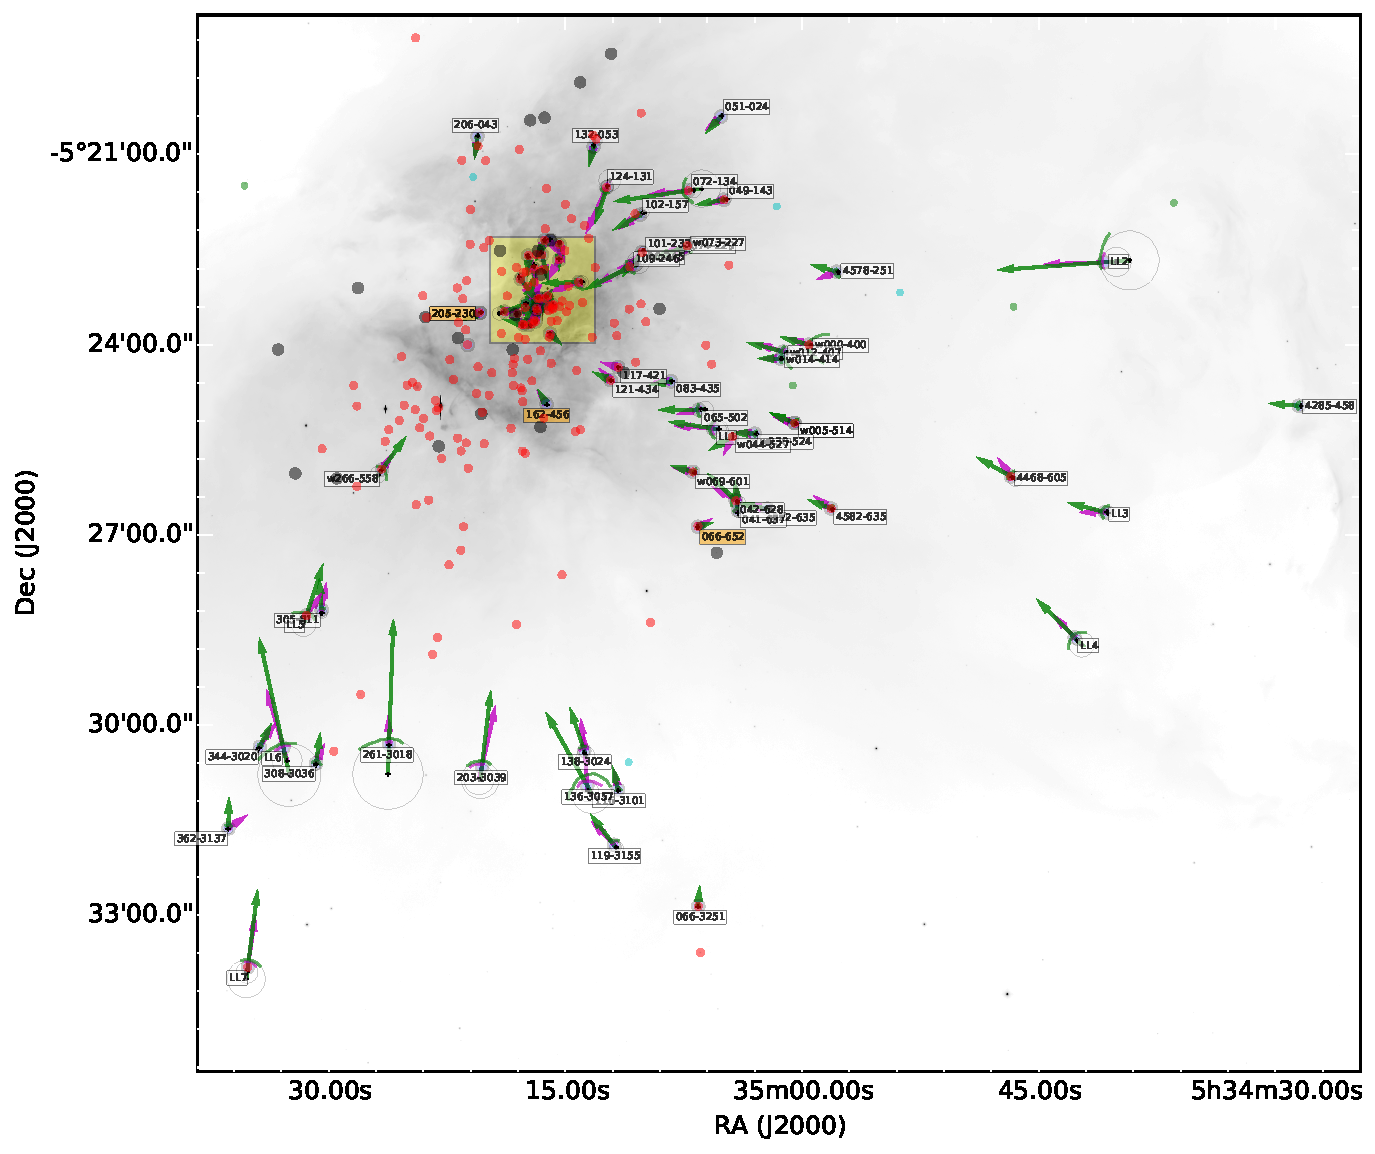
\includegraphics[width=\linewidth]{ll-pos-image}
  \caption{Position of bow shock arcs.}
  \label{fig:pos-image}
\end{figure*}

\begin{figure*}
  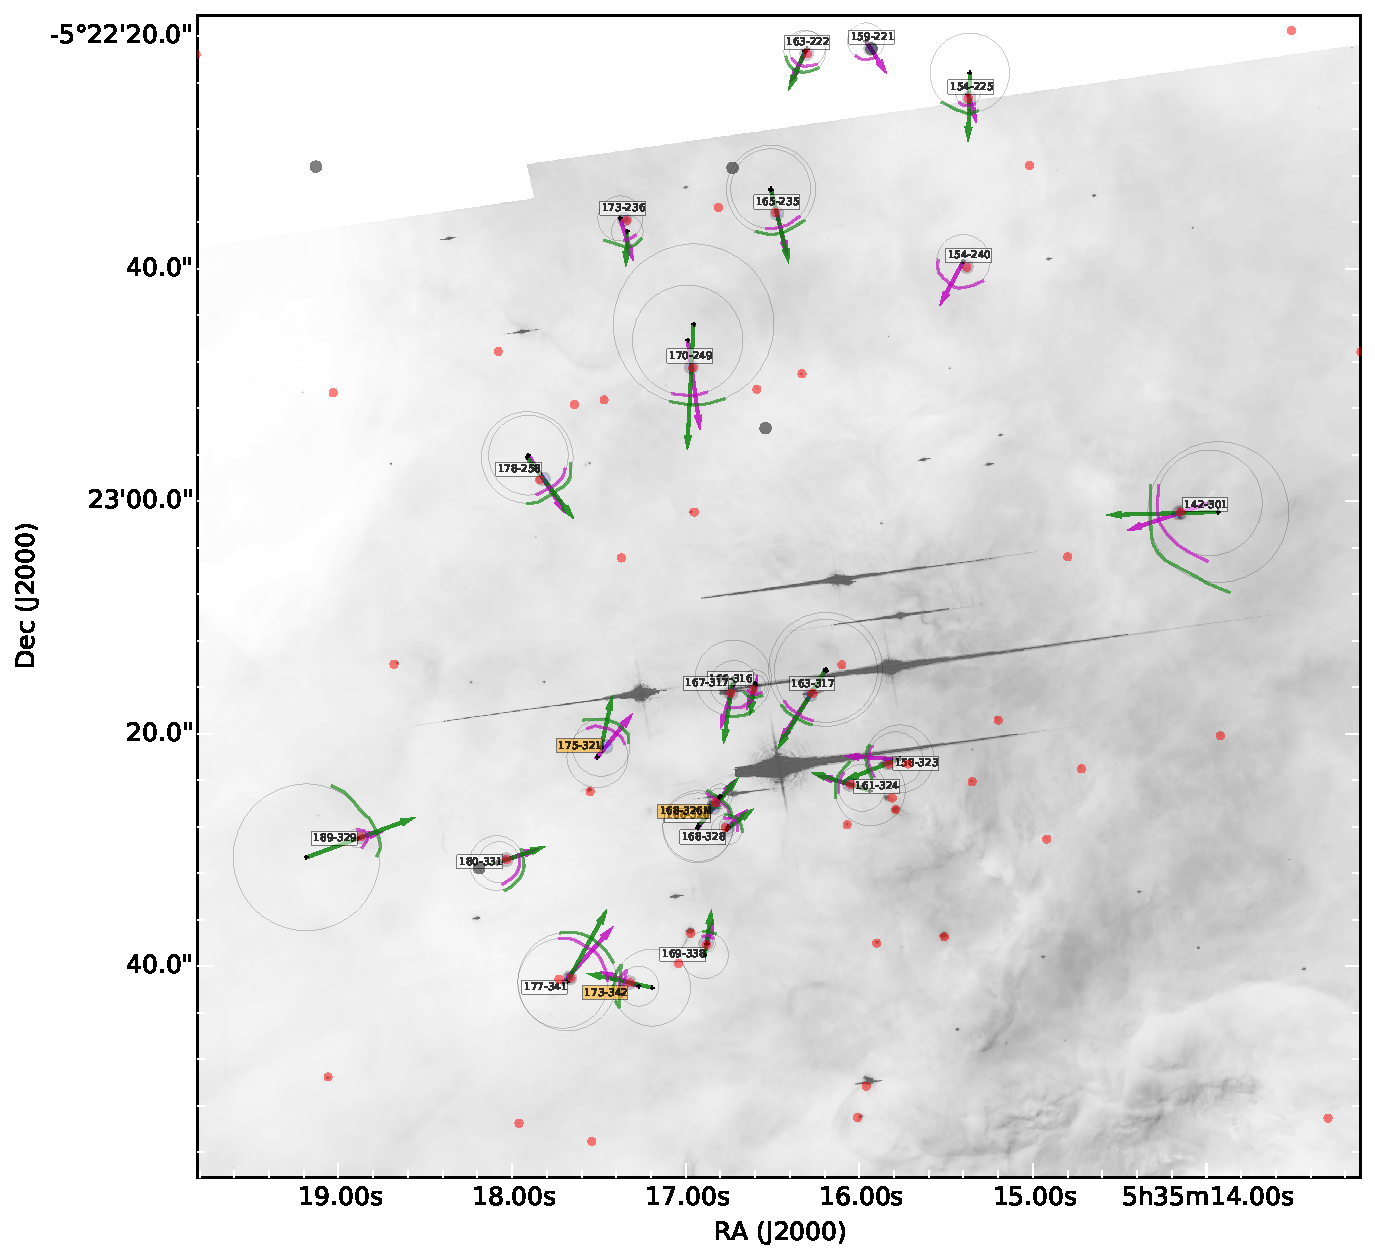
\includegraphics[width=\linewidth]{ll-pos-image-zoom}
  \caption{Position of bow shock arcs. Zoomed area.}
  \label{fig:pos-image}
\end{figure*}

\begin{figure*}
  \centering
  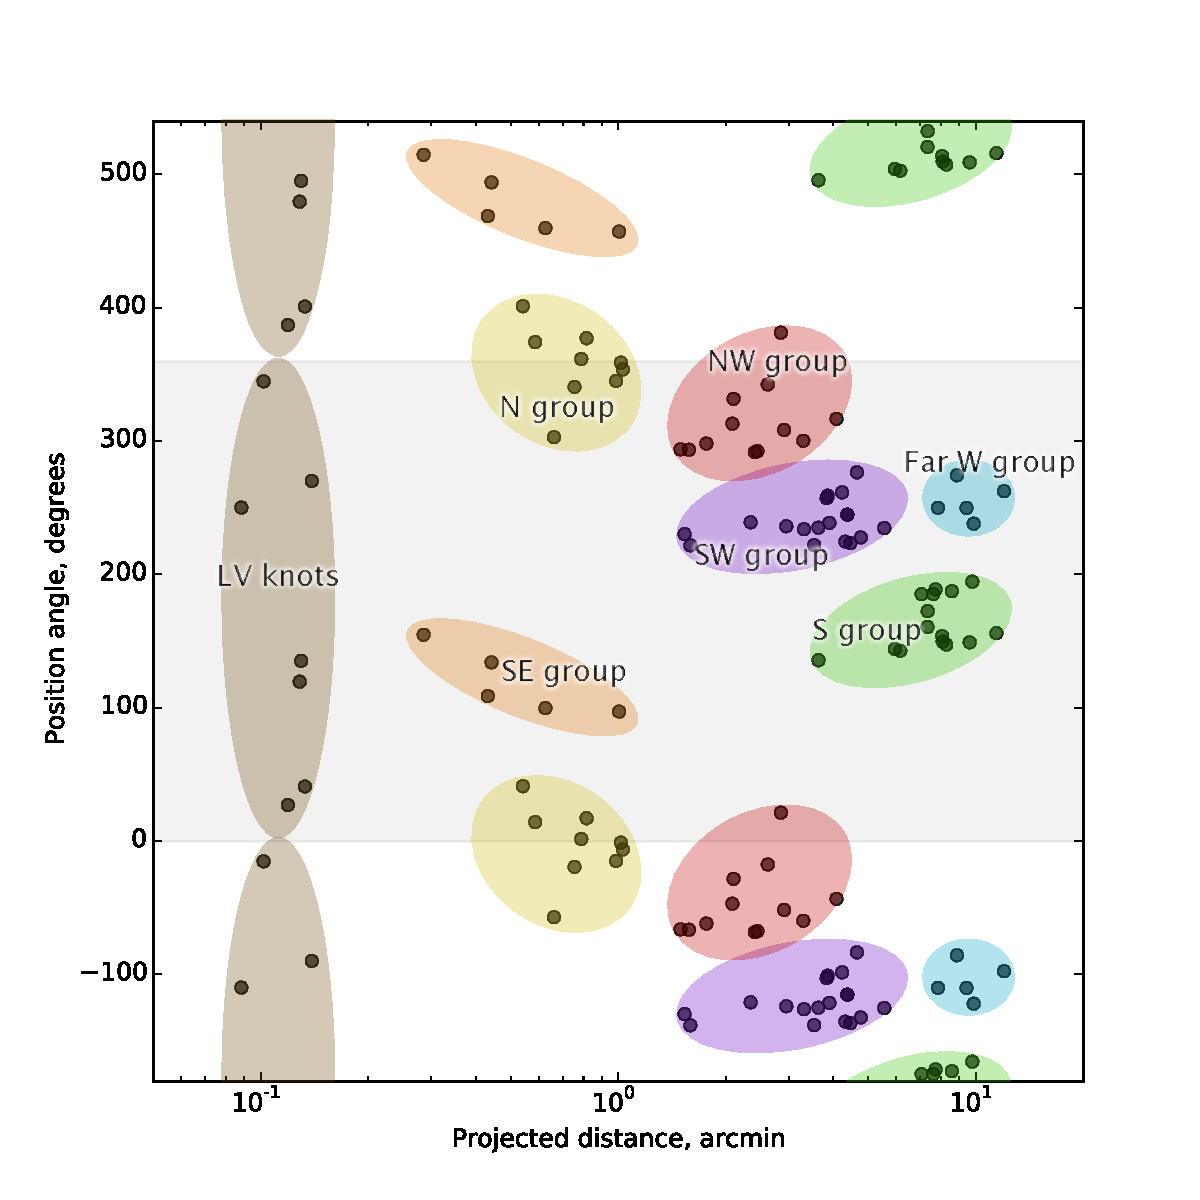
\includegraphics[width=\linewidth]{arc-classify}
  \caption{Spatial distribution of the bowshock arcs and classification into spatial groups.}
  \label{fig:size-v-distance}
\end{figure*}

\section{Catalog}
\label{sec:catalog}

\subsection{LV knot group}
\label{sec:lv-group}
\input{table-sort-01-LV.tex}
\input{fig-stamps-01-LV.tex}

\clearpage
\subsection{Southeast group}
\label{sec:se-group}
\input{table-sort-02-southeast.tex}
\input{fig-stamps-02-southeast.tex}

\clearpage
\subsection{North group}
\label{sec:n-group}
\input{table-sort-03-north.tex}
\input{fig-stamps-03-north.tex}

\clearpage
\subsection{Northwest group}
\label{sec:nw-group}
\input{table-sort-04-northwest.tex}
\input{fig-stamps-04-northwest.tex}

\clearpage
\subsection{Southwest group}
\label{sec:sw-group}
\input{table-sort-05-southwest.tex}
\input{fig-stamps-05-southwest.tex}

\clearpage
\subsection{West group}
\label{sec:w-group}
\input{table-sort-06-west.tex}
\input{fig-stamps-06-west.tex}

\clearpage
\subsection{South group}
\label{sec:s-group}
\input{table-sort-07-south.tex}
\input{fig-stamps-07-south.tex}

\clearpage
\subsection{Interproplyd shells}
\label{sec:interproplyd-group}
\input{table-sort-00-interproplyd.tex}
\input{fig-stamps-00-interproplyd.tex}

\clearpage
\subsection{probably not shells}
\label{sec:problematic-group}
\input{table-sort-XX-problematic.tex}
\input{fig-stamps-XX-problematic.tex}

\clearpage
\section{Discussion}
\label{sec:discuss}
\begin{figure}
  (\textit{a})\\
  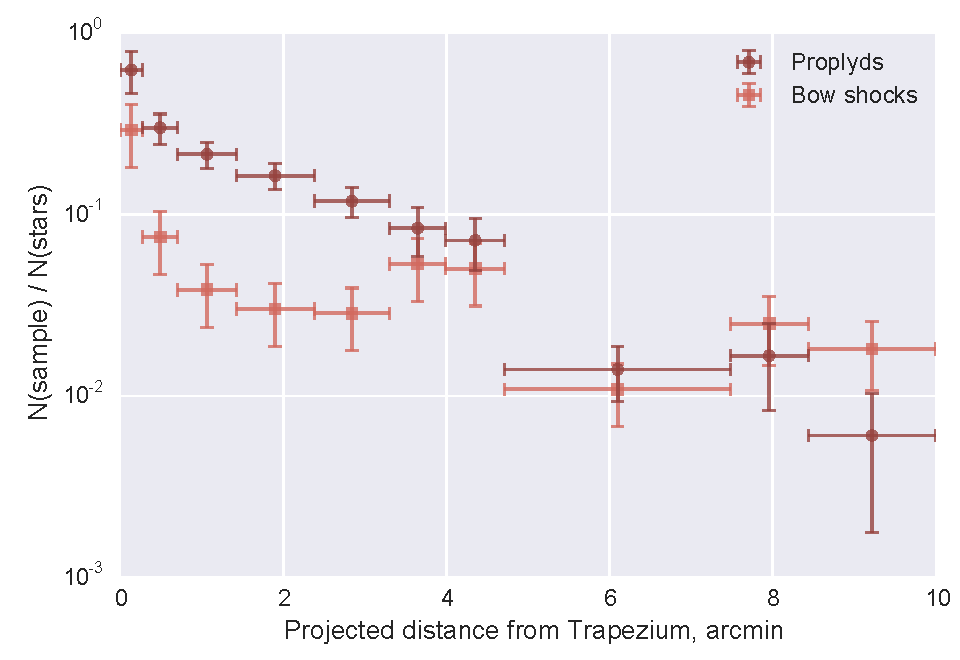
\includegraphics[width=\linewidth]{proplyd-star-ratio}\\
  (\textit{b})\\
  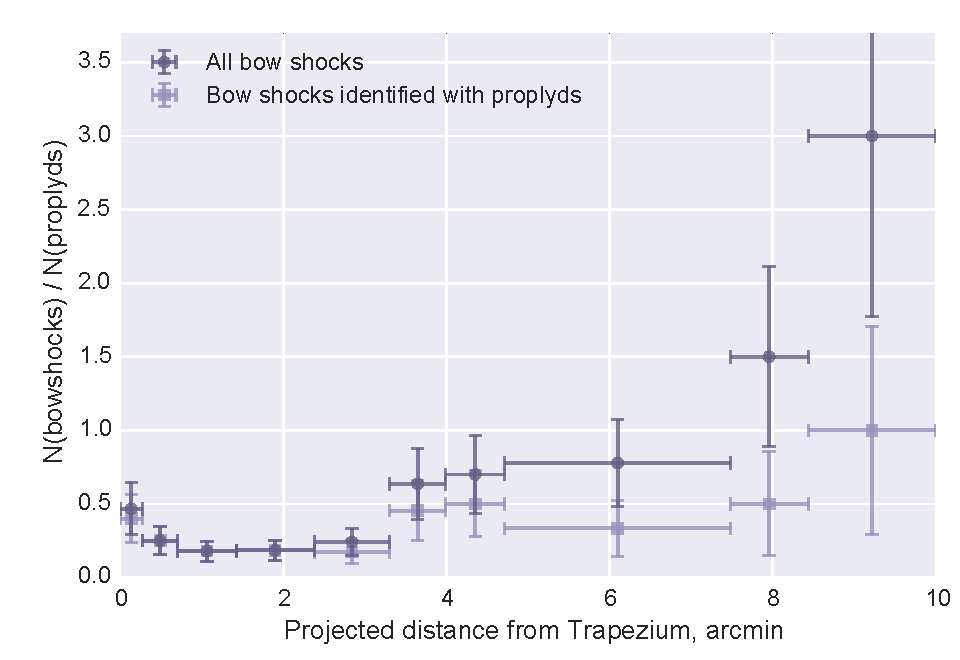
\includegraphics[width=\linewidth]{bowshock-proplyd-ratio}
  \caption{(\textit{a})~Fraction of all optically visible stars that
    are proplyds (dark circle symbols) or have bowshocks (light square
    symbols) as a function of projected separation from the Trapezium.
    (\textit{b})~Ratio between number of bowshocks and number of
    proplyds as a function of projected separation from the Trapezium.
    Dark circle symbols show all bowshocks in our catalog (with the
    exception of interproplyd shocks) while light square symbols show
    only those bowshocks associated with known or suspected proplyds.
  }
  \label{fig:bow-proplyd-star-ratios}
\end{figure}

Proplyd over star fraction falls off relatively smoothly with projected distance.  Albeit with a sudden drop after about 200 arcsec.


Bowshock over proplyd fraction seems to have three separate peaks.   Very small distances corresponding to the wind-wind interaction, then there is a dearth of bowshocks until a second peak around four arcmin.  Finally at very large radii there may be a third peak of objects that are not proplyds.

But an alternate explanation for the third peak could be that they are all proplyds but that the proplyd fraction is underestimated at large distances.

On the other hand there is also evidence for three distinct populations from the azimuthal distribution around the Trapezium.  The group at 4 arcmin separation are mainly to the west whereas the more distant objects are mainly to the south.


\begin{figure}
  \centering
  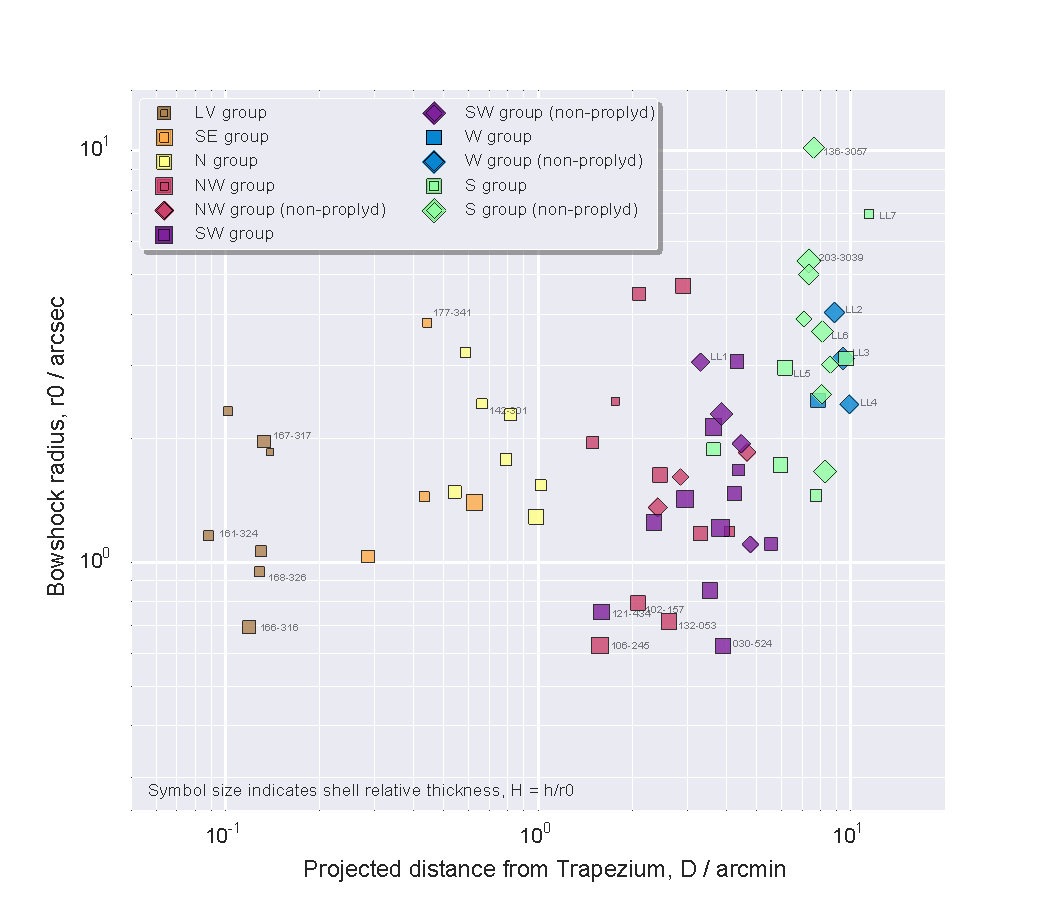
\includegraphics[width=\linewidth]{will-r0-vs-D-class}
  \caption{Bowshock axial size versus distance from the Trapezium.}
  \label{fig:size-v-distance}
\end{figure}
\begin{figure}
  \centering
  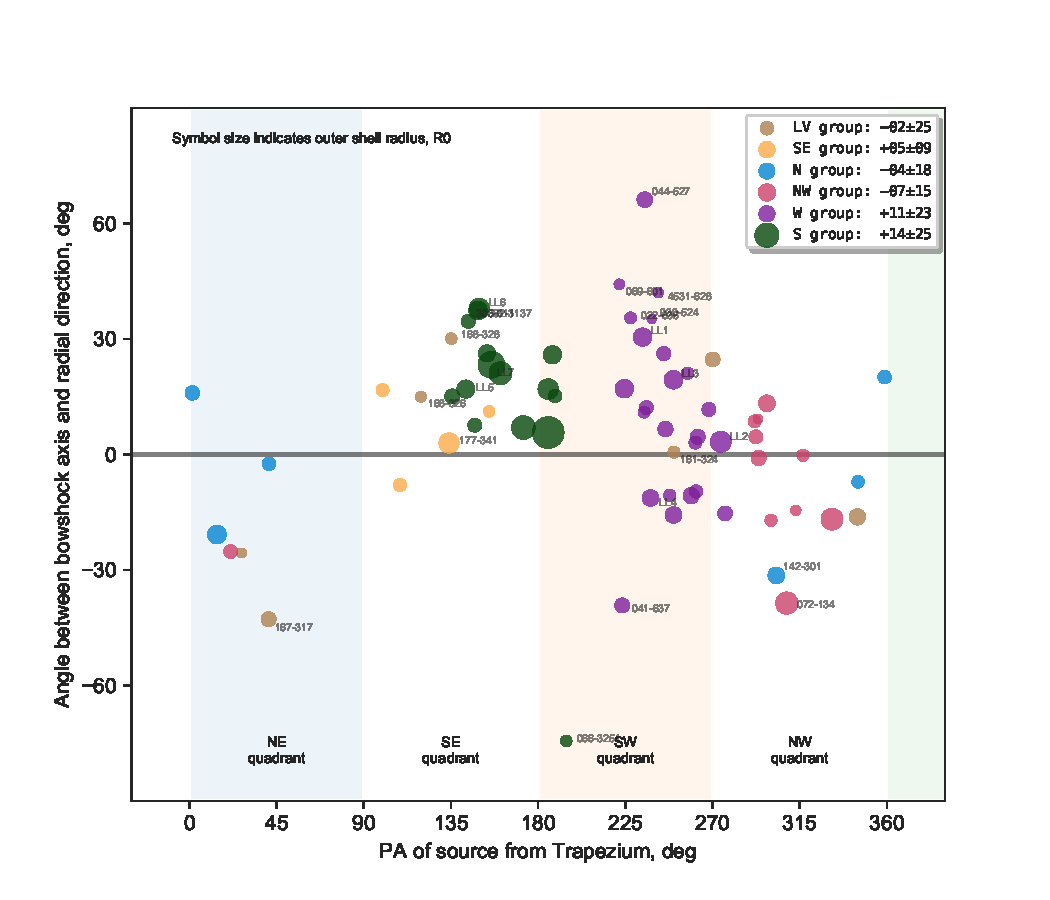
\includegraphics[width=\linewidth]{will-PA-vs-PA-class}
  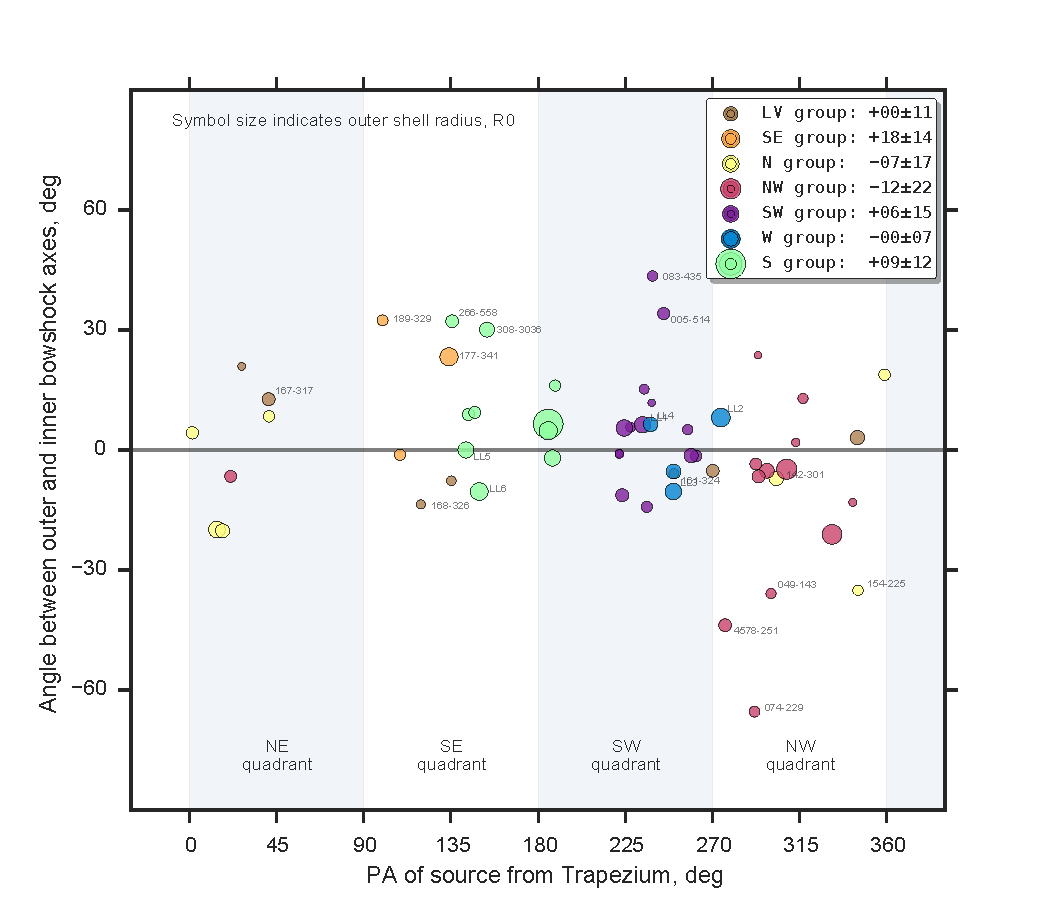
\includegraphics[width=\linewidth]{will-PA-out-vs-in-class}
  \caption{Angle offset between bowshock axis and the radial direction to \thC{} .}
  \label{fig:PA-v-PA}
\end{figure}
\begin{figure}
  \centering
  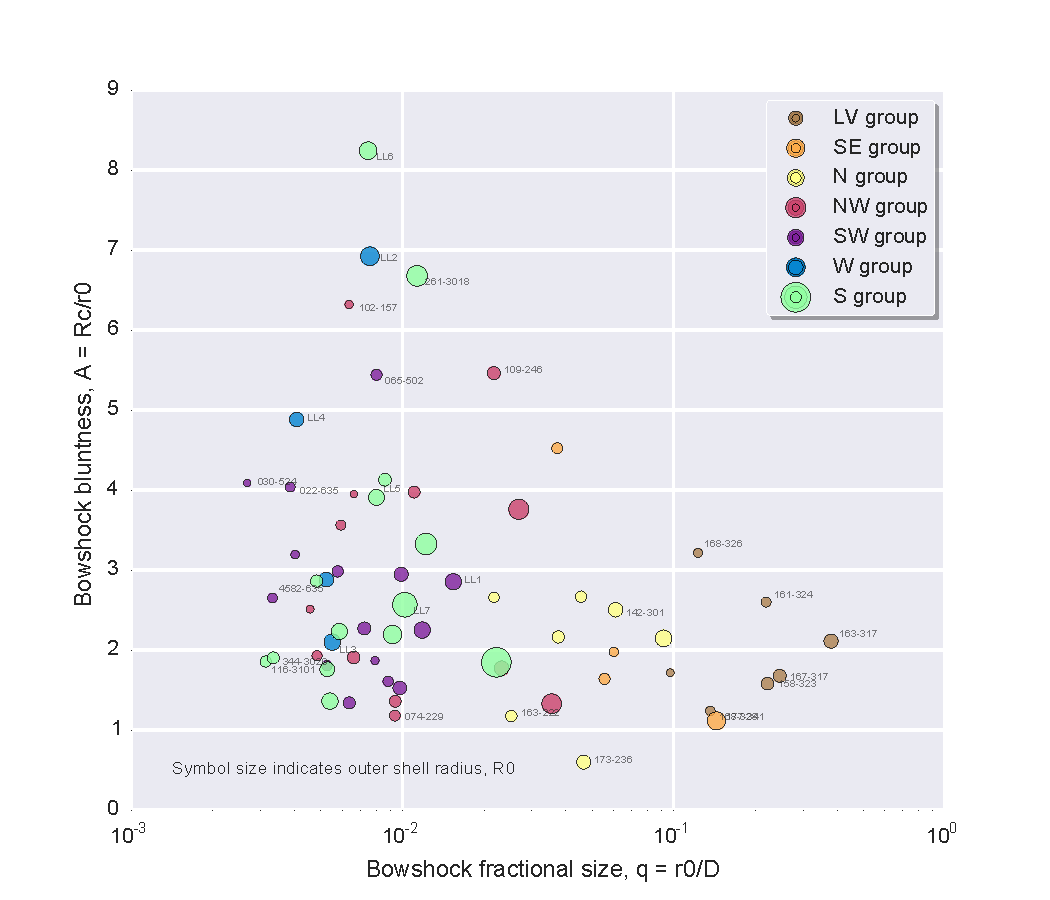
\includegraphics[width=\linewidth]{will-A-vs-q-class}
  \caption{Bowshock bluntness versus relative size.}
  \label{fig:A-v-q}
\end{figure}
\begin{figure}
  \centering
  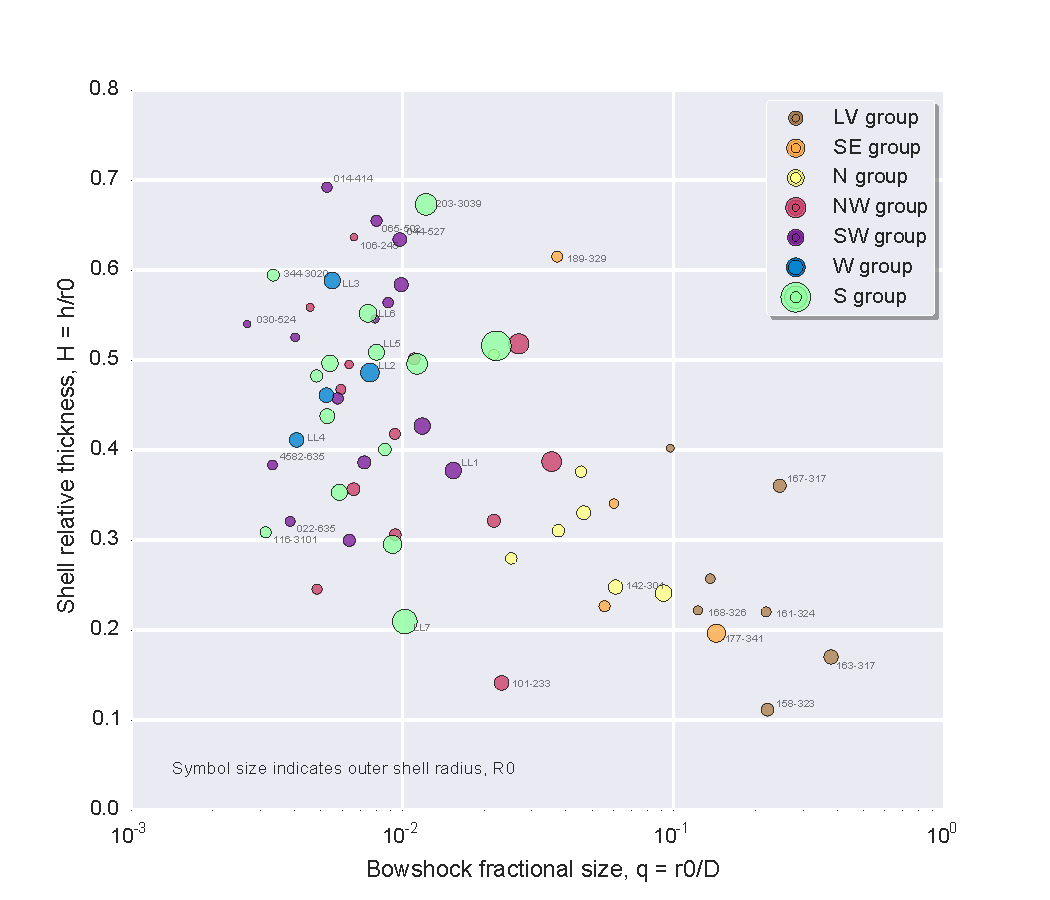
\includegraphics[width=\linewidth]{will-H-vs-q-class}
  \caption{Bowshock relative shell thickness versus relative size.}
  \label{fig:PA-v-PA}
\end{figure}

\bibliography{BibdeskLibrary-slavoj}


\end{document}
